% !TEX root = ./report.tex

\clearpage
\section{The Regionalized Value State Dependence Graph}
\label{background:RVSDG}

The \textit{Regionalized Value State Dependence Graph}~\cite{RVSDG:HiPEACpaper}
(RVSDG) is a \textit{directed acyclic demand-based dependence graph},
consisting of nodes representing computations and edges representing the
dependencies between nodes. Each node has inputs and outputs connected through
edges. The arity and order of inputs and outputs depend on the operation the
node represents.

Figure~\ref{fig:simple_node_RVSDG_ex} exemplifies how the C/C++ code on the left
can be represented as an RVSDG. The nodes in
Figure~\ref{fig:simple_node_RVSDG_ex} represent operations in a program, while
the edges between the nodes show the dependencies nodes have to each other, thus
giving the order of execution.

In all RVSDG examples depicted in this report, the order of inputs in a node
goes clockwise. The first input of a node is the one closest to the bottom left
corner of the node.

\begin{centering}
	\noindent\begin{minipage}{0.36\textwidth}
		\begin{CenteredBox}
		\begin{lstlisting}[label={lst:simple_node_RVSDG_ex},
style=minipage_customcpp, basicstyle=\fontsize{10}{1}]
x = (y*2) / (z+2);
		\end{lstlisting}
		\end{CenteredBox}
	\end{minipage}
	\noindent\begin{minipage}{0.55\textwidth}
		\captionsetup{type=figure}
		\includegraphics[width=\textwidth]{figures/simple_node_RVSDG_ex}
	\end{minipage}
	\captionof{figure}{Example of an RVSDG subgraph equivalent to the C/C++
on the left.}
	\label{fig:simple_node_RVSDG_ex}
\end{centering}

\subsection{Edges}

The RVSDG has data dependence edges and state dependence edges, representing
data and state dependencies operations have to each other, respectively. An
example of data dependence edges are the operands used in an addition, such as
in Figure~\ref{fig:simple_node_RVSDG_ex}.

State dependence edges are used to preserve the semantics of the program when
the program has side-effecting operations. If there are no data dependencies
between operations, state dependence edges can give the needed order of
execution. Figure~\ref{fig:load_dependence_ex} illustrates the use of state
dependence edges, depicted as dotted edges.

\begin{centering}
	\noindent\begin{minipage}{0.36\textwidth}
		\begin{CenteredBox}
		\begin{lstlisting}[label={lst:load_dependence_ex},
style=minipage_customcpp, basicstyle=\fontsize{10}{1}]
*x += 7;
*y += 7;
		\end{lstlisting}
		\end{CenteredBox}
	\end{minipage}
	\noindent\begin{minipage}{0.55\textwidth}
		\captionsetup{type=figure}
		\includegraphics[width=\textwidth]{figures/load_store_state_dependence_ex}
	\end{minipage}
	\captionof{figure}{Example of an RVSDG subgraph equivalent to the C/C++
on the left.}
	\label{fig:load_dependence_ex}
\end{centering}

The \textit{S}-node in Figure~\ref{fig:load_dependence_ex} supplies the needed
state edge for \lstinline!x!'s \textit{load}- and \textit{store}-nodes.

\subsection{Nodes}

The RVSDG has two kinds of nodes: simple nodes and complex nodes. The arity and
order of inputs and outputs of any RVSDG node need to match the operation.

\subsubsection{Simple Nodes}

Simple nodes are used to represent primitive operations, such as addition and
substraction. Figure~\ref{fig:simple_node_RVSDG_ex} is an example of an RVSDG
containing only simple nodes.

One simple node of special interest for this report is the \applyNode . An
\applyNode~represents the call site of a function. The first input argument of
an \applyNode~is the function the \applyNode~invokes. The remaining inputs are
the arguments to this function. Likewise, its results are the results of the
invocation of its function. Order and arity of inputs and outputs need to match
the arguments and results of the funtion, respectively.

\subsubsection{Complex Nodes}

Complex nodes contain one or more RVSDG subgraphs, which is why they are also
referred to as \textit{regions}. Differing from the simple nodes with their
contained subgraph, complex nodes may besides the normal inputs and outputs,
also have internal inputs and outputs. Figure~\ref{fig:complex_node_mapping_ex}
shows which inputs/outputs are the external ones, and which are the internal
ones. Figure~\ref{fig:complex_node_mapping_ex} also illustrates how the values
of the external inputs are mapped to the internal outputs of each subregion, and
vica versa with each subregion's internal inputs being mapped to the external
outputs.

\begin{figure}[H]
	\centering
	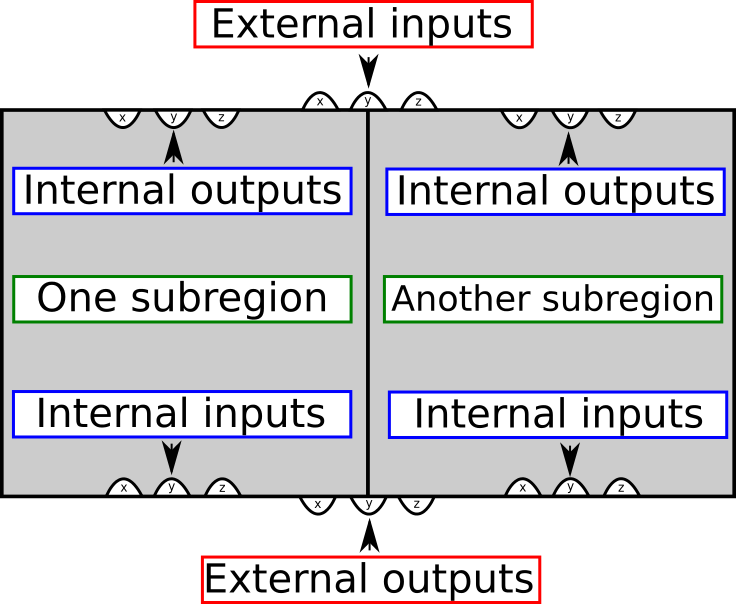
\includegraphics[width=0.7\textwidth]{figures/complex_node_mapping_ex}
	\caption{A minimal example of a complex node, showing which inputs/outputs
are external/internal, and how they can have multiple subregions.}
	\label{fig:complex_node_mapping_ex}
\end{figure}

As Figure~\ref{fig:complex_node_mapping_ex} also shows, some complex nodes may
also have multiple \textit{subregions}. If a complex node has more than one
subregion, the arity and order of all the internal inputs/outputs must match
between all subregions, as well as match the arity and order of the external
inputs/outputs of the complex node.

The complex nodes of an RVSDG relevant for this report are as follows:

\begin{itemize}

\item \textbf{$\gamma$-nodes: N-way statements}

\textit{$\gamma$-nodes} represent conditional statements. Each $\gamma$-node has
a predicate as first input. All other edges passing as inputs to the
$\gamma$-node are edges its subregions depend upon. Each subregion represents
one case. All subregions must have the same order and arity of internal inputs
and outputs, even if the subgraph in each region does not depend on all of the
internal outputs.

A $\gamma$-node is equivalent to a \textit{switch-case} without fall-through in
C/C++. Each case of the switch statement corresponds to a subregion of the
$\gamma$-node. Hence, a simple \textit{if-statement} with no else-clause can be
represented by a $\gamma$-node with two subregions. The true subregion contains
the RVSDG subgraph that represents the body of the if-statement, whereas the
false subregion of the $\gamma$-node simply routes all inputs through. See
Figure~\ref{fig:simple_if} for an example of a $\gamma$-node.

\begin{centering}
	\noindent\begin{minipage}{0.36\textwidth}
		\begin{CenteredBox}
		\begin{lstlisting}[label={lst:simple_if}, style=minipage_customcpp,
basicstyle=\fontsize{10}{1}]
if((z-2) != 0 ){
	x = (y*2) / (z+2);
}
		\end{lstlisting}
		\end{CenteredBox}
	\end{minipage}
	\noindent\begin{minipage}{0.55\textwidth}
		\captionsetup{type=figure}
		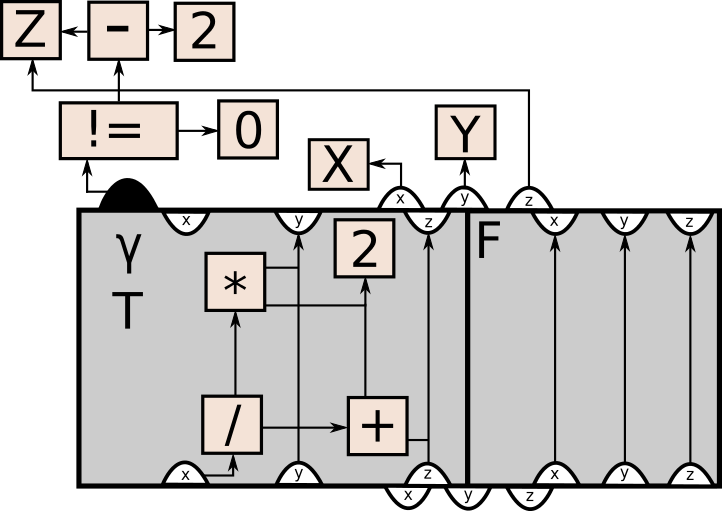
\includegraphics[width=\textwidth]{figures/simple_if_example}
	\end{minipage}
	\captionof{figure}{Example of an RVSDG subgraph on the right, depicting a
$\gamma$-node equivalent to the C/C++ if-statement on the left.}
	\label{fig:simple_if}
\end{centering}

\item \textbf{$\theta$-nodes: Tail-controlled loops}

\textit{$\theta$-nodes} represent tail-controlled loops. As with
$\gamma$-nodes, its inputs (and outputs) are all the dependencies needed for the
RVSDG subgraph in its subregion.

The first time the body of the loop is executed, the external inputs are
mapped to the internal outputs, as Figure~\ref{fig:factorial_loop_ex}
exemplifies. This enables the complex node's contained RVSDG subgraph to
execute with the values given as external inputs to the $\theta$-node.

However, inside the $\theta$-node there is an extra first internal input, which
is the predicate of the tail-controlled loop. If this predicate evaluates to
\lstinline!true!, the rest of the internal inputs of the $\theta$-node are
mapped to their corresponding internal outputs. This enables the iterative
behaviour of an RVSDG $\theta$-node. Thus, the operations represented by its
contained RVSDG subgraph are executed as a tail-controlled loop. Finally, when
the predicate evaluates to false, the internal inputs are mapped to the external
outputs of the $\theta$-node instead of the internal outputs.

A $\theta$-node is equivalent to a \textit{do-while} loop in C/C++, as shown in
Figure~\ref{fig:factorial_loop_ex}.

\begin{centering}
	\noindent\begin{minipage}{0.36\textwidth}
		\begin{CenteredBox}
		\begin{lstlisting}[style=minipage_customcpp,
label={lst:fig:factorial_loop_ex}, basicstyle=\fontsize{10}{1}]
unsigned int i = 0;
unsigned long r = 1;
do {
	i += 1;
	r *= i;
} while(i < n);
		\end{lstlisting}
		\end{CenteredBox}
	\end{minipage}
	\noindent\begin{minipage}{0.55\textwidth}
		\captionsetup{type=figure}
		\includegraphics[width=\textwidth]{figures/iterative_factorial_ex}
	\end{minipage}
	\captionof{figure}{An RVSDG subgraph on the right, depicting a
$\theta$-node equivalent to the C/C++ do-while loop on the left.}
	\label{fig:factorial_loop_ex}
\end{centering}

A \textit{head-controlled} loop can be represented by putting a $\theta$-node
inside the subregion representing the \textit{true } clause of a $\gamma$-node.
Additionally, both the $\gamma$-node's first input and the first internal input
of the $\theta$-node need to share the same predicate. Finally, the
$\gamma$-node's subregion representing the \textit{false} clause cannot contain
nodes.

\item \textbf{$\lambda$-nodes: Functions}

\textit{$\lambda$-nodes} represent functions. A $\lambda$-node contains an RVSDG
subgraph representing the body of a function. The internal inputs of a
$\lambda$-node represents the results of the function. Respectively, its
internal outputs represent the arguments of the function. While $\lambda$-nodes
don't have any external inputs, their external output are what give the
\applyNode s their first input, enabling them to invoke the function represented
by the $\lambda$-node.

The arity and order of a $\lambda$-node's internal inputs and outputs must match
the arity and order of the external inputs and outputs of all connected
\applyNode s.

Hence, when an \applyNode~connected with a $\lambda$-node is executed, the
external inputs of the \applyNode~are mapped to the internal outputs of the
$\lambda$-node, before the $\lambda$-node is invoked.

Likewise the internal inputs of the $\lambda$-node are mapped to the external
outputs of the \applyNode~when the operations of the $\lambda$-node have been
executed. See Figure~\ref{fig:iterative_factorial_func_ex} for an example of a
$\lambda$-node.

\begin{centering}
	\noindent\begin{minipage}{0.37\textwidth}
		\begin{CenteredBox}
		\begin{lstlisting}[label={lst:iterative_factorial_func_ex},
style=minipage_customcpp, basicstyle=\fontsize{10}{1}]
unsigned long long
fac(unsigned int n){
	unsigned int i = 0;
	unsigned long r = 1;
	do{
		i += 1;
		r *= i;
	} while(i < n);
	return r;
}
		\end{lstlisting}
		\end{CenteredBox}
	\end{minipage}
	\noindent\begin{minipage}{0.55\textwidth}
		\captionsetup{type=figure}
		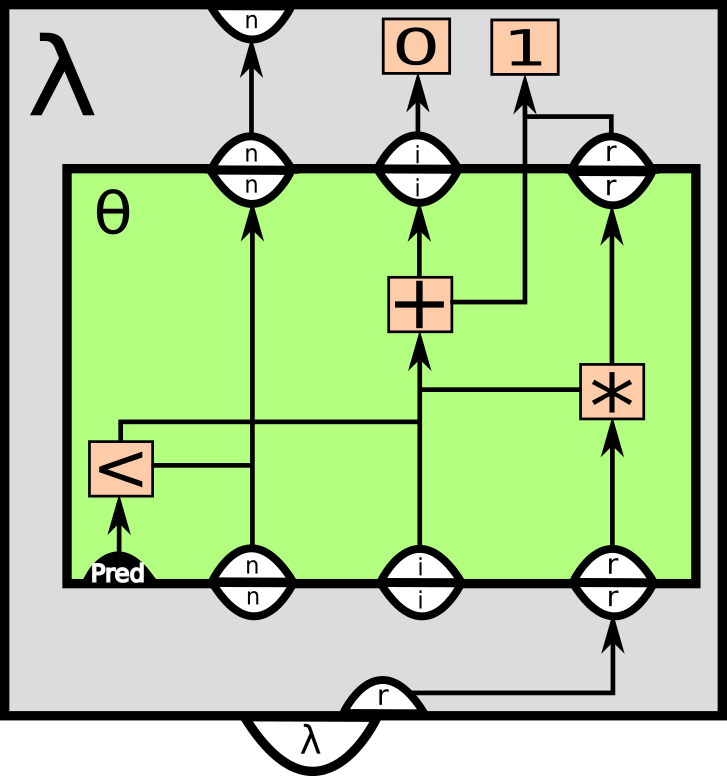
\includegraphics[width=\textwidth]{figures/iterative_factorial_func_ex}
	\end{minipage}
	\captionof{figure}{Example of an RVSDG subgraph on the right, depicting a
$\lambda$-node equivalent to the C/C++ function on the left.}
	\label{fig:iterative_factorial_func_ex}
\end{centering}

\item \textbf{$\phi$-regions: Recursive environments}

\textit{$\phi$-regions} represent recursive environments. They contain at least
one recursive $\lambda$-node. Like the $\lambda$-node, they have no external
inputs. However, the internal outputs of the $\phi$-region represent the links
utilized by the \applyNode s contained within to connect with the respective
$\lambda$-nodes.

The internal inputs of a $\phi$-region receive the function invocation links
from the $\lambda$-nodes contained within. The internal inputs map to the
external outputs, thus enabling \applyNode s outside of the recursive
environment to connect with the $\lambda$-nodes, as depicted in
Figure~\ref{fig:recursive_factorial_func_ex}.

\begin{centering}
	\noindent\begin{minipage}{0.37\textwidth}
		\begin{CenteredBox}
		\begin{lstlisting}[label={lst:recursive_factorial_func_ex},
style=minipage_customcpp, basicstyle=\fontsize{10}{1}]
unsigned long long
fac(unsigned int n){
	unsigned long r  = 1;
	if(n > 1){
		r = n*fac(n-1);
	}
	return r;
}
		\end{lstlisting}
		\end{CenteredBox}
	\end{minipage}
	\noindent\begin{minipage}{0.55\textwidth}
		\captionsetup{type=figure}
		\includegraphics[width=\textwidth]{figures/recursive_factorial_func_ex}
	\end{minipage}
	\captionof{figure}{Example of an RVSDG subgraph on the right, depicting a
$\phi$-region equivalent to the recursive C/C++function on the left.}
	\label{fig:recursive_factorial_func_ex}
\end{centering}

\end{itemize}
